\subsection*{Traditional Extrapolation Methods}
Before we begin to develop in full the SRE method for determining the converged CCD correlation energies with respect to the number of single-particle states in the calculation, let us look at two traditional methods for removing the basis incompleteness error and two methods that may work based on the analysis from the last section.

%% TRUNCATE
The most common way to deal with a basis incompleteness error is to truncate the number of single-particle states at some high number. Fig. \ref{fig:compare_no_sre} displays the results of truncating the calculations at 20 open shells, corresponding to between 922 and 2,090 single particle states depending on the number of electrons in the calculation for a HEG with $r_s$ = 0.5. This graph, plotted in orange, is compared to the correlation energy calculation performed at 70 total energy shells (M = 6,142) in black, which are the fully converged results where the basis incompleteness error is eliminated. Of course, one way to negate the basis incompleteness error is to perform calculations at very high numbers of single-particle states. However, as we saw in the last section, this is not necessarily feasible due to the high computational time and resource requirements, and, therefore, simply increasing the number of single-particle states in the system is not an attractive option for removing the basis incompleteness error.

%% POWER LAW
Another common method is to find the correlation energy in the complete basis limit by using a power law of the form:

\begin{equation}
    \Delta E_{CCD}(M) = E_{CCD,\infty} + AM^{-\alpha},
\end{equation}

where $E_{CCD,\infty}$ (the correlation energy in the complete basis limit) and A are fit to data from correlation energy calculations at several different values of M. The value of $\alpha$ is typically fixed to 1, so this method is generally referred to as a 1/M power law (REFERENCE HERE). The results of performing this power law fit on a HEG system with $r_s$ = 0.5 and using 16 data points per number of electrons (from 5 open shells to 20 open shells) are shown in Fig. \ref{fig:compare_no_sre} in blue.  We can see that this power law fit overestimates the HEG correlation energies by about the same margin that the truncation at 20 open shells underestimated them. This indicates that for the data available, neither of these traditional methods of removing the basis incompleteness error are attractive option. The power law does not provide a good fit and overestimates the correlation energies; while truncating the basis at a large number of single-particle states can provide an accurate result, the computational time and resource requirements make this option not feasible for many systems.

%% SLOPE at SET SHELL NUMBER
Next, we can look at two methods inspired by the analysis performed in the previous section. In Fig. \ref{mbpt_vs_cc}, the graph is reasonably linear if we plot the CCD correlation energies as a function of the MBPT2 correlation energies. The first approach to calculating the converged CCD correlation energies from this plot may be to take the CCD and MBPT2 calculation at a relatively high number of single-particle states, create the ratio $m = \Delta E_{CCD}/\Delta E_{MBPT2}$, and then take m and multiply it by the MBPT2 correlation energy at a very high number of single-particle states to approximate the CCD correlation energy at that same high number of single-particle states (here M = 6,142): $\Delta E_{CCD, 6142} \approx m\Delta E_{MBPT2, 6142}$. For this investigation, we derived the slope from calculations performed at 20 open energy shells (the same truncation level we used earlier), then calculated the slope and generated a prediction for the CCD correlation energy at 6,142 single-particle states. This analysis's results are shown in green in Fig. \ref{fig:compare_pnm_all_no_sre}. We can see that this is a much better approximation of the converged CCD correlation energies than the previous two attempts. However, there are still significant deviations at higher numbers of electrons. Therefore, while this is an improvement, we will seek a better method to accurately predict the converged correlation energies at all numbers of electrons, including the high values.

%% LINEAR REGRESSION
As a final method, we will use linear regression to fit a subset of the data shown in Fig. \ref{mbpt_vs_cc}.  It should be noted that even though machine learning is quite a simple machine learning algorithm, this is our first machine learning approach to remove the basis incompleteness error from these calculations.

For training the linear regression algorithm, we will use 16 sets of MBPT2 and CCD correlation energies drawn from calculations between 5 and 20 open shells (the exact number of single-particle states depends on the number of electrons). First, the linear regression algorithm will be trained and then asked to predict $\Delta E_{CCD, 6142}$ by giving $\Delta E_{MBPT2,6142}$. It is important to remember that generating MBPT2 correlation energies is a fast computation.

The results of performing this analysis are shown in red in Fig. \ref{fig:compare_no_sre}. These results are similar to the previous slope analysis, where the correlation energies at lower numbers of electrons are well matched, but there are deviations at higher numbers. We could improve this result by using training data drawn from higher M values. However, like the other methods shown here, that is an unattractive solution due to the increased computational time and resource requirements.

%% ERROR COMPARISON AND CONCLUSION

Thus the two traditional extrapolation methods we have looked at and the two new methods fail to satisfactorily remove the basis incompleteness errors without requiring data drawn from calculations with a much higher number of single-particle states. Thus, we need to be in a position to begin fully developing the SRE method.

\begin{figure}
    \centering
    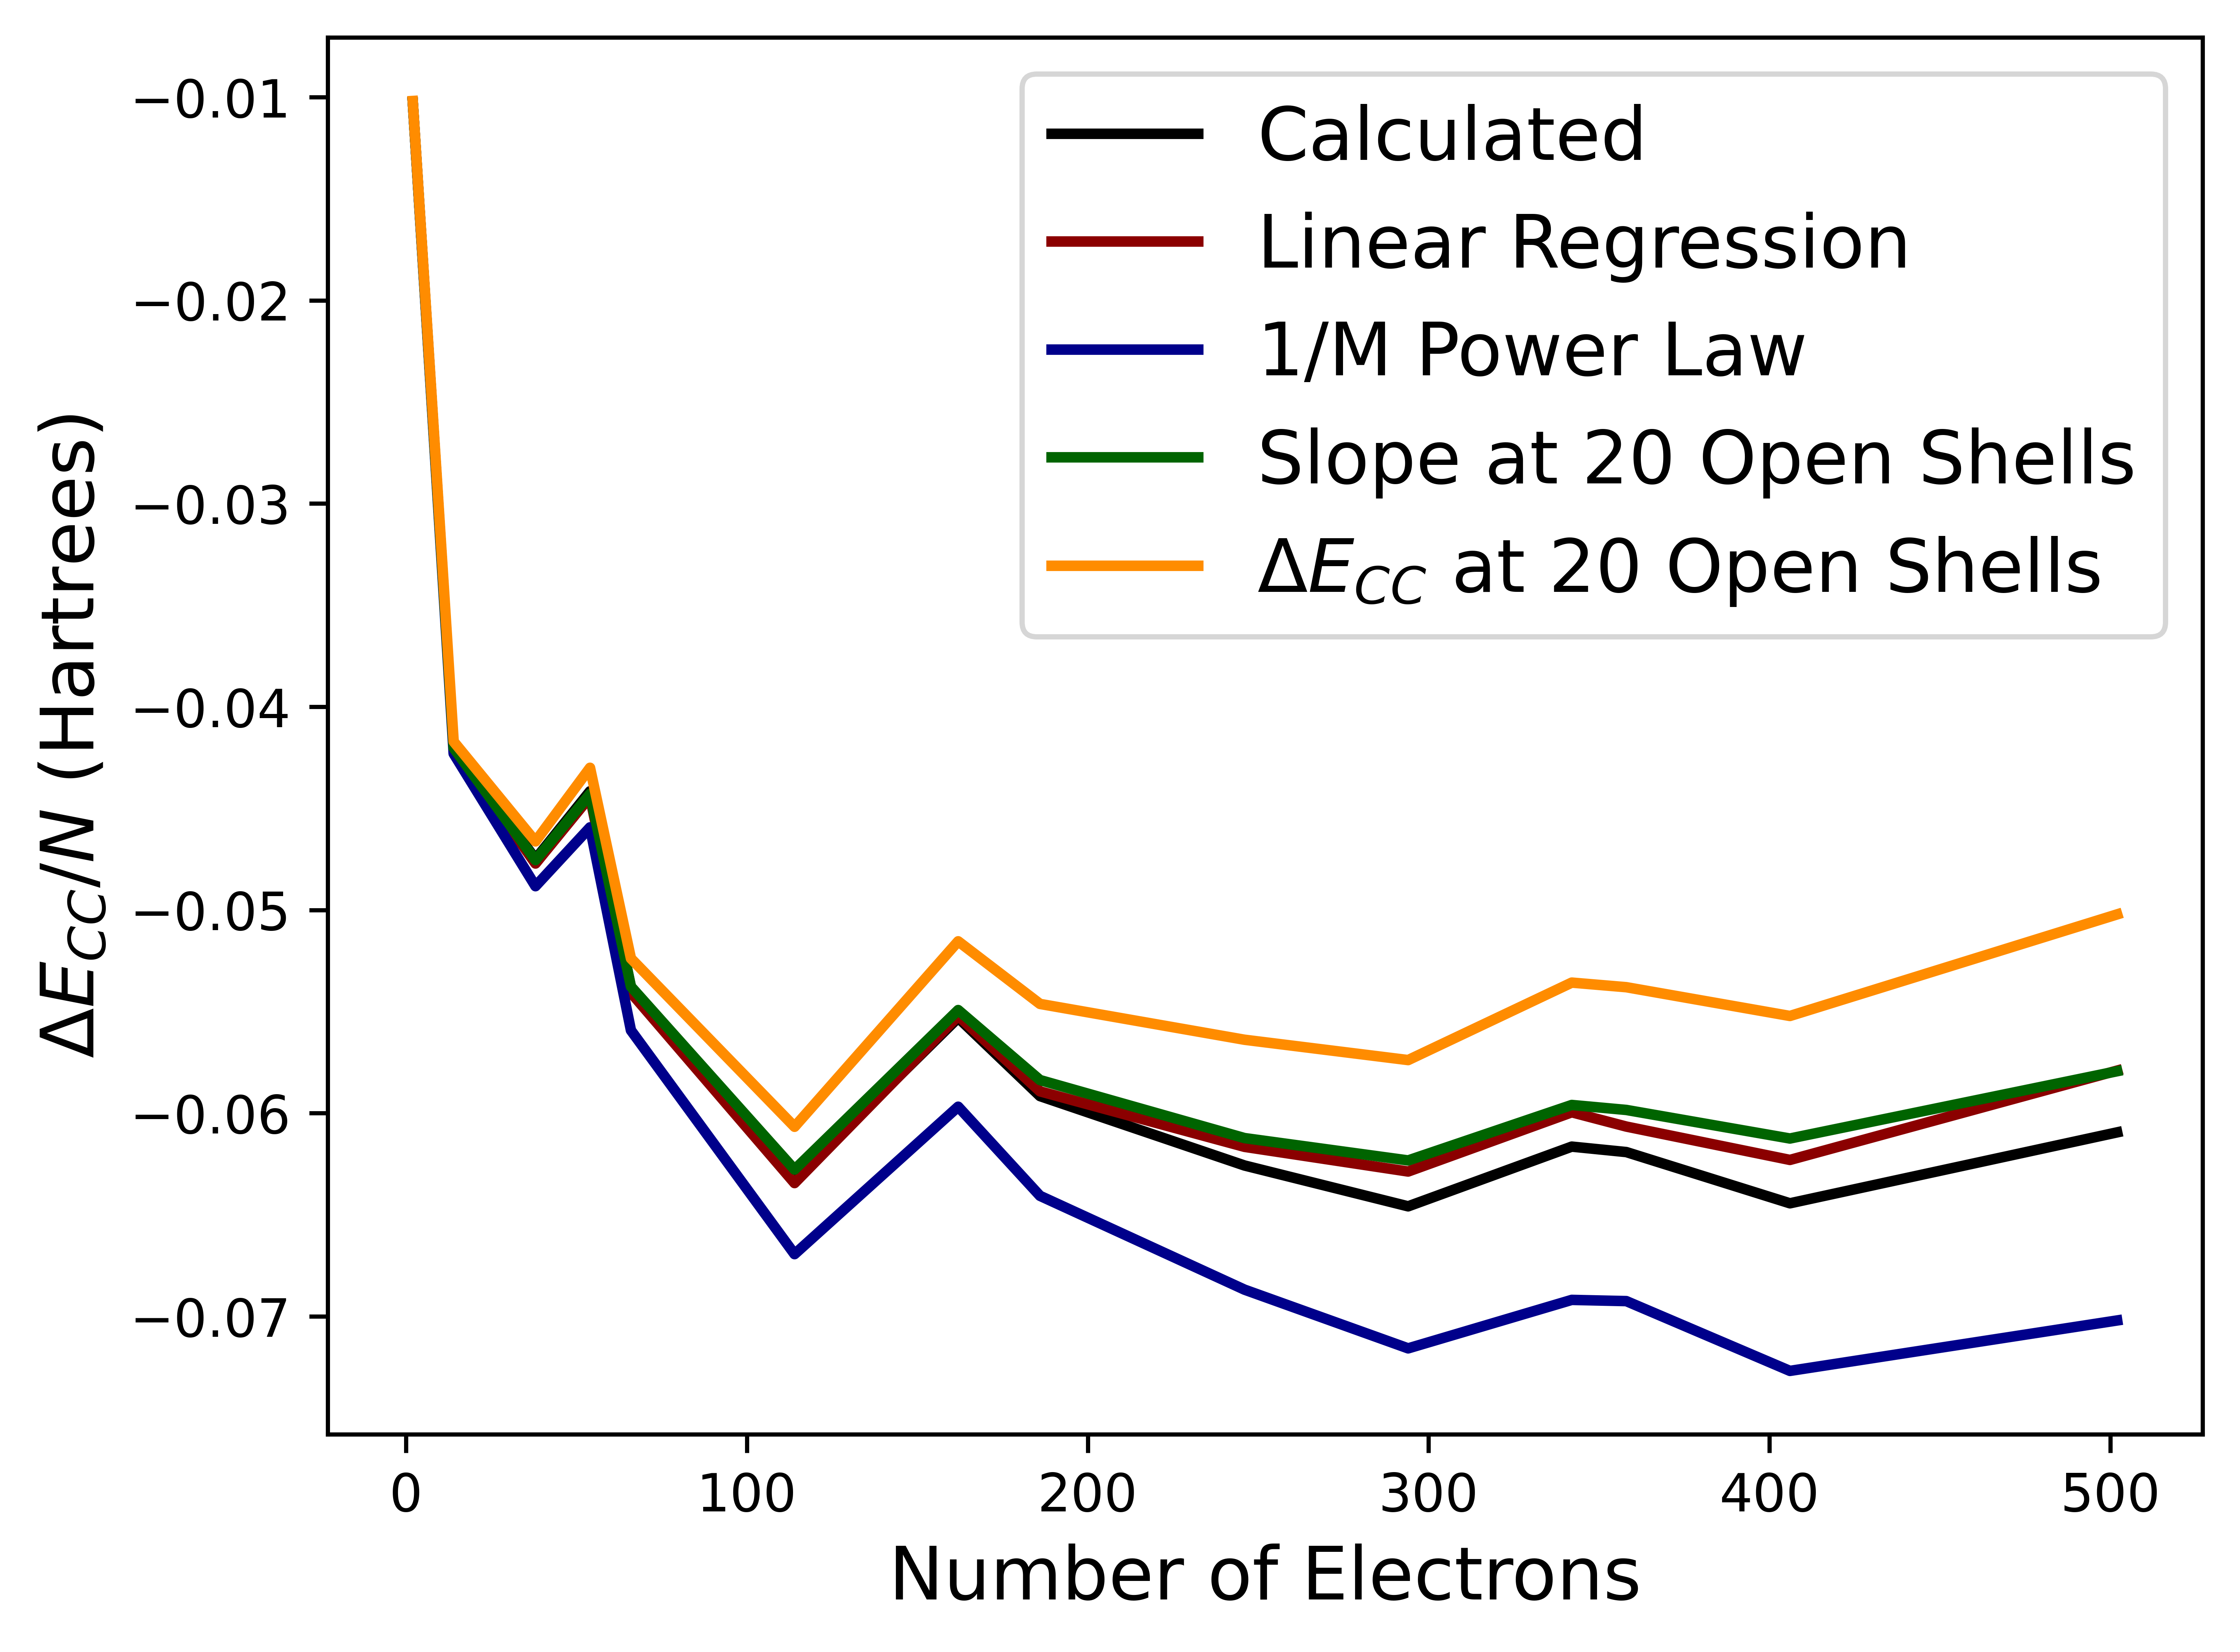
\includegraphics[scale=0.75]{Images/Chapter7/ElectronGas/EG_extrapolation_compare_no_sre.png}
    \caption{The converged CCD correlation energies (black) calculated at M = 6,142 for an HEG with $r_s$ = 0.5.  Also displayed are the results of predicting the converged correlation energies with a truncation at 20 open shells (yellow) which has a percent error of 6.87$\%$, using a 1/M power law (blue) which has an average percent error of 7.00$\%$, using the CCD to MBPT2 slope calculated at 20 open shells (green) which have an average percent error of 1/16$\%$, and using linear regression to model the graph from Fig. \ref{mbpt_vs_cc} (red) which has an average percent error of 0.95$\%$.}
    \label{fig:compare_no_sre}
\end{figure}